\documentclass{article}
\usepackage{amsmath}
\usepackage{amsfonts}
\usepackage{geometry}
\usepackage{xcolor}
\usepackage{graphicx}
\usepackage{hyperref}
\usepackage{booktabs} % Add this to your preamble for the table

\geometry{a4paper, margin=1in}

\begin{document}

\title{Kinematics Part I: Definitions and Diagrams}
\author{}
\date{}
\maketitle

\section{Core Definitions}

Kinematics is the study of motion without considering its causes. We define the state of motion using three fundamental vectors. In this handout, we use $d$ (and $\vec{d}$) for displacement throughout.

\subsection*{1.1 Position and Displacement}
\begin{itemize}
  \item \textbf{Position ($\vec{r}$ or $\vec{x}$):} A vector representing the location of an object relative to an origin $O$.
  \item \textbf{Displacement ($\Delta \vec{d}$):} Defined as the change in position. It is the straight-line vector from the starting point to the ending point: $\Delta \vec{d} = \vec{r}_f - \vec{r}_i$.
\end{itemize}

\subsection*{1.2 Velocity ($\vec{v}$)}
Velocity is the rate of change of displacement. \textbf{Average velocity} is defined as:
\begin{equation}
  \vec{v}_{\text{av}} = \frac{\Delta \vec{d}}{\Delta t}
  \label{eq:v_avg}
\end{equation}

\textbf{Instantaneous velocity} describes the motion at an instant, this will be covered after you learn calculus.
\begin{equation}
  \vec{v} = \frac{d\vec{x}}{dt}
  \label{eq:v_inst}
\end{equation}

\textit{Note: Here $dx$ and $dt$ are differentials from calculus, and they are not the same as the displacement $\vec{d}$.}

\subsection*{1.3 Acceleration ($\vec{a}$)}
Acceleration is the rate of change of velocity. For \textbf{uniform acceleration}, the (constant) acceleration is:
\begin{equation}
  \vec{a} = \frac{\Delta \vec{v}}{\Delta t} = \frac{\vec{v}_f - \vec{v}_i}{\Delta t}
  \label{eq:accel_def}
\end{equation}

\newpage

\section{The \texorpdfstring{$v\text{--}t$}{v-t} Diagram (Velocity-Time)}

The $v-t$ diagram is a fundamental tool because its geometric properties correspond directly to physical quantities.
\begin{figure}[htp]
  \centering
  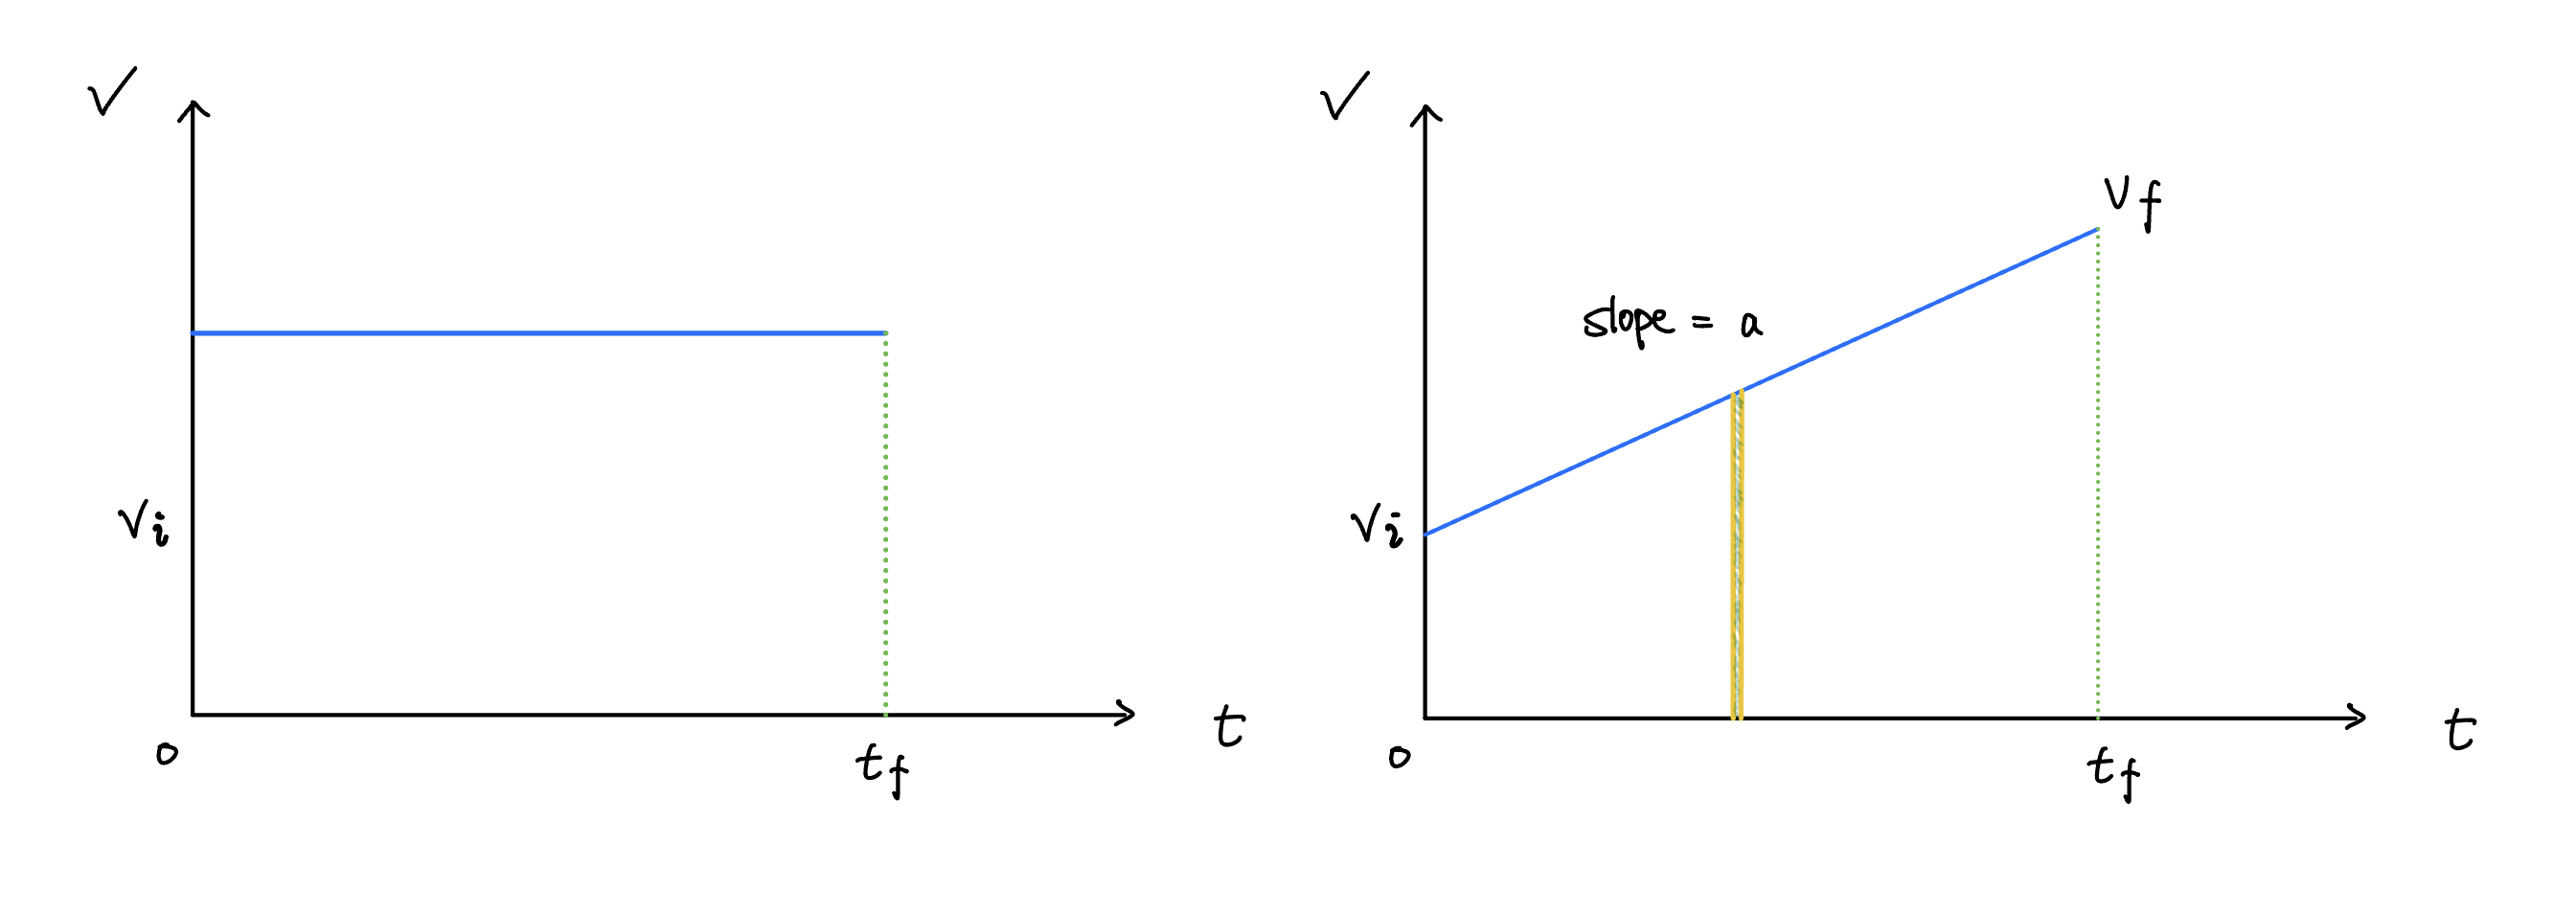
\includegraphics[width=15cm]{v_t_diagram.png}
  \label{fig:v_t_diagram}
  \caption{v-t. diagram for uniform motion and uniform acceleration motion}
\end{figure}

\subsection{Why is the Slope equal to Acceleration?}
By definition, acceleration is $\vec{a} = \frac{\Delta \vec{v}}{\Delta t}$. In a $v-t$ coordinate system:
\begin{itemize}
  \item The vertical change is $\Delta v$ (rise).
  \item The horizontal change is $\Delta t$ (run).
\end{itemize}
Since $\text{Slope} = \frac{\text{rise}}{\text{run}} = \frac{\Delta v}{\Delta t}$, the \textbf{slope} of a $v-t$ graph represents the \textbf{acceleration}.

\subsection{Why is the Area equal to Displacement?}
\subsubsection*{Constant Velocity}
From Eq.~\eqref{eq:v_avg}, for constant velocity, $\Delta d = v \Delta t$. This geometrically forms a \textbf{rectangle} with height $v$ and width $\Delta t$. Thus, $\text{Area} = \text{Displacement}$ (signed area).

\subsubsection*{Changing Velocity (The "Slicing" Logic)}
For an object with changing velocity, we divide the total time into many extremely small intervals $dt$:
\begin{itemize}
  \item During each tiny interval, the velocity is nearly constant.
  \item The displacement for that slice is the area of a very thin rectangle ($v_{\text{slice}} \cdot dt$).
  \item The total displacement is the sum of all these tiny areas, filling the entire space under the curve.
\end{itemize}
Conclusion: The \textbf{area under the curve} in a $v-t$ diagram represents the \textbf{total displacement} $\Delta \vec{d}$ (signed area).

\newpage
\section{Uniform Acceleration Equations}

For motion with constant acceleration, we derive the core equations:

\subsection{The Velocity Equation}
\begin{equation}
  v_f = v_i + a\Delta t
  \label{eq:ua:v_final}
\end{equation}
\textbf{Derivation:} Rearranging the definition of acceleration in Eq.~\eqref{eq:accel_def}: $\Delta v = a\Delta t \Rightarrow v_f - v_i = a\Delta t$.

\subsection{The Displacement Equation (Missing \texorpdfstring{$v_f$}{v\_f})}
\begin{equation}
  \Delta d = v_i \Delta t + \frac{1}{2}a(\Delta t)^2
  \label{eq:ua:disp_1}
\end{equation}
\textbf{Derivation:} The total area under the $v-t$ slope is a trapezoid, which can be split into:
\begin{enumerate}
  \item A \textbf{Rectangle}: Area $= v_i \cdot \Delta t$.
  \item A \textbf{Triangle}: Area $= \frac{1}{2} \cdot \Delta t \cdot \Delta v$.
\end{enumerate}
Substituting $\Delta v = a\Delta t$ from Eq.~\eqref{eq:ua:v_final} into the triangle area yields the result.

\subsection{The Average Velocity Equation (Missing \texorpdfstring{$a$}{a})}
\begin{equation}
  \Delta d = \left( \frac{v_i + v_f}{2} \right) \Delta t
  \label{eq:ua:v_avg_disp}
\end{equation}
\textbf{Derivation:} Geometrically, the area of a trapezoid is $\frac{1}{2}(\text{top} + \text{bottom}) \times \text{height}$.

\subsection{The Time-Independent Equation (Missing \texorpdfstring{$\Delta t$}{Delta t})}
\begin{equation}
  v_f^2 = v_i^2 + 2a\Delta d
  \label{eq:ua:time_indep}
\end{equation}
\textbf{Derivation:} Isolate $\Delta t = \frac{v_f - v_i}{a}$ from Eq.~\eqref{eq:ua:v_final} and substitute it into Eq.~\eqref{eq:ua:v_avg_disp}.

\subsection{The Alternative Displacement Equation (Missing \texorpdfstring{$v_i$}{v\_i})}
\begin{equation}
  \Delta d = v_f \Delta t - \frac{1}{2}a(\Delta t)^2
  \label{eq:ua:disp_2}
\end{equation}

\newpage

\section{The Five-Step Method for Kinematics}

To solve motion problems systematically, follow these five steps:

\begin{description}
  \item[1. Set Positive Direction] \hfill \\
    Establish a coordinate system (e.g., denote right or up as $+$). All vectors ($\Delta d, v, a$) must be assigned signs relative to this convention.
  \item[2. Draw the $v-t$ Diagram] \hfill \\
    Sketch the velocity-time graph. This identifies if the motion is multi-stage (e.g., acceleration followed by constant velocity) and helps verify if your final displacement should be positive or negative.
  \item[3. Identify Variables (The Inventory)] \hfill \\
    List the five kinematic variables: $\{v_i, v_f, a, \Delta t, \Delta d\}$. Fill in the given values (with signs!) and mark the target unknown with a ``?''.
  \item[4. Select the Equation] \hfill \\
    Identify the ``missing variable'' (the one neither given nor required) and choose the corresponding equation from the table below.
  \item[5. Solve and Check] \hfill \\
    Rearrange the equation algebraically before plugging in numbers. Ensure units are consistent ($m, s, m/s$) and the sign of the result makes physical sense.
\end{description}

\subsection*{Equation Selection Guide (The Big Five)}
\begin{table}[h]
  \centering
  \begin{tabular}{llc}
    \toprule
    \textbf{Equation} & \textbf{Missing Variable} \\ \midrule
    $v_f = v_i + a\Delta t$ & $\Delta d$ \\
    $\Delta d = v_i\Delta t + \frac{1}{2}a(\Delta t)^2$ & $v_f$ \\
    $v_f^2 = v_i^2 + 2a\Delta d$ & $\Delta t$ \\
    $\Delta d = \left( \frac{v_i + v_f}{2} \right) \Delta t$ & $a$ \\
    $\Delta d = v_f \Delta t - \frac{1}{2}a(\Delta t)^2$ & $v_i$ \\ \bottomrule
  \end{tabular}
\end{table}

\end{document}
